%% BioMed_Central_Tex_Template_v1.06
%%                                      %
%  bmc_article.tex            ver: 1.06 %
%                                       %

%%IMPORTANT: do not delete the first line of this template
%%It must be present to enable the BMC Submission system to
%%recognise this template!!

%%%%%%%%%%%%%%%%%%%%%%%%%%%%%%%%%%%%%%%%%
%%                                     %%
%%  LaTeX template for BioMed Central  %%
%%     journal article submissions     %%
%%                                     %%
%%          <8 June 2012>              %%
%%                                     %%
%%                                     %%
%%%%%%%%%%%%%%%%%%%%%%%%%%%%%%%%%%%%%%%%%

%%%%%%%%%%%%%%%%%%%%%%%%%%%%%%%%%%%%%%%%%%%%%%%%%%%%%%%%%%%%%%%%%%%%%
%%                                                                 %%
%% For instructions on how to fill out this Tex template           %%
%% document please refer to Readme.html and the instructions for   %%
%% authors page on the biomed central website                      %%
%% https://www.biomedcentral.com/getpublished                      %%
%%                                                                 %%
%% Please do not use \input{...} to include other tex files.       %%
%% Submit your LaTeX manuscript as one .tex document.              %%
%%                                                                 %%
%% All additional figures and files should be attached             %%
%% separately and not embedded in the \TeX\ document itself.       %%
%%                                                                 %%
%% BioMed Central currently use the MikTex distribution of         %%
%% TeX for Windows) of TeX and LaTeX.  This is available from      %%
%% https://miktex.org/                                             %%
%%                                                                 %%
%%%%%%%%%%%%%%%%%%%%%%%%%%%%%%%%%%%%%%%%%%%%%%%%%%%%%%%%%%%%%%%%%%%%%

%%% additional documentclass options:
%  [doublespacing]
%  [linenumbers]   - put the line numbers on margins

%%% loading packages, author definitions

%\documentclass[twocolumn]{bmcart}% uncomment this for twocolumn layout and comment line below
\documentclass{bmcart}

%%% Load packages
\usepackage{amsthm,amsmath}
\usepackage{fancyvrb}
\DefineVerbatimEnvironment{Code}{Verbatim}{}
\DefineVerbatimEnvironment{CodeInput}{Verbatim}{fontshape=sl}
\DefineVerbatimEnvironment{CodeOutput}{Verbatim}{}
\newenvironment{CodeChunk}{}{}
%\RequirePackage[numbers]{natbib}
%\RequirePackage[authoryear]{natbib}% uncomment this for author-year bibliography
%\RequirePackage{hyperref}
\usepackage[utf8]{inputenc} %unicode support
\usepackage{graphicx} 
%\usepackage[applemac]{inputenc} %applemac support if unicode package fails
%\usepackage[latin1]{inputenc} %UNIX support if unicode package fails

%%%%%%%%%%%%%%%%%%%%%%%%%%%%%%%%%%%%%%%%%%%%%%%%%
%%                                             %%
%%  If you wish to display your graphics for   %%
%%  your own use using includegraphic or       %%
%%  includegraphics, then comment out the      %%
%%  following two lines of code.               %%
%%  NB: These line *must* be included when     %%
%%  submitting to BMC.                         %%
%%  All figure files must be submitted as      %%
%%  separate graphics through the BMC          %%
%%  submission process, not included in the    %%
%%  submitted article.                         %%
%%                                             %%
%%%%%%%%%%%%%%%%%%%%%%%%%%%%%%%%%%%%%%%%%%%%%%%%%

%\def\includegraphic{}
%\def\includegraphics{}

%%% Put your definitions there:
\startlocaldefs
\endlocaldefs

%%% Begin ...
\begin{document}

%%% Start of article front matter
\begin{frontmatter}

\begin{fmbox}
\dochead{Databases}

%%%%%%%%%%%%%%%%%%%%%%%%%%%%%%%%%%%%%%%%%%%%%%
%%                                          %%
%% Enter the title of your article here     %%
%%                                          %%
%%%%%%%%%%%%%%%%%%%%%%%%%%%%%%%%%%%%%%%%%%%%%%

\title{A Compressed Large Language Model Embedding Dataset of ICD 10 CM 
Descriptions}

%%%%%%%%%%%%%%%%%%%%%%%%%%%%%%%%%%%%%%%%%%%%%%
%%                                          %%
%% Enter the authors here                   %%
%%                                          %%
%% Specify information, if available,       %%
%% in the form:                             %%
%%   <key>={<id1>,<id2>}                    %%
%%   <key>=                                 %%
%% Comment or delete the keys which are     %%
%% not used. Repeat \author command as much %%
%% as required.                             %%
%%                                          %%
%%%%%%%%%%%%%%%%%%%%%%%%%%%%%%%%%%%%%%%%%%%%%%

\author[
  addressref={aff1},                   % id's of addresses, e.g. {aff1,aff2}
  corref={aff1},                       % id of corresponding address, if any
% noteref={n1},                        % id's of article notes, if any
  email={michael.kane@yale.edu}   % email address
]{\inits{M.J.}\fnm{Michael J.} \snm{Kane}}
\author[
  addressref={aff2,aff3},
  email={casey.king@yale.edu}
]{\inits{C.}\fnm{Casey} \snm{King}}
\author[
  addressref={aff1},
  email={denise.esserman@yale.edu}
]{\inits{D.}\fnm{Denise} \snm{Esserman}}
\author[
  addressref={aff4},
  email={nklatham@bwh.harvard.edu}
]{\inits{N.K.}\fnm{Nancy K.} \snm{Latham}}
\author[
  addressref={aff1},
  email={erich.greene@yale.edu}
]{\inits{E.}\fnm{Erich J.} \snm{Greene}}
\author[
  addressref={aff5},
  email={dganz@mednet.ucla.edu}
]{\inits{D.A.}\fnm{David A.} \snm{Ganz}}

%%%%%%%%%%%%%%%%%%%%%%%%%%%%%%%%%%%%%%%%%%%%%%
%%                                          %%
%% Enter the authors' addresses here        %%
%%                                          %%
%% Repeat \address commands as much as      %%
%% required.                                %%
%%                                          %%
%%%%%%%%%%%%%%%%%%%%%%%%%%%%%%%%%%%%%%%%%%%%%%

\address[id=aff1]{%                           % unique id
  \orgdiv{Department of Biostatistics},       % department, if any
  \orgname{School of Public Health},          % university, etc
  \street{Yale University},
  \city{New Haven},                              % city
  \cny{USA}                                    % country
}
\address[id=aff2]{%
  \orgdiv{The Jackson School of Global Affairs}
  \orgname{Yale University},
  %\street{},
  %\postcode{}
  \city{New Haven},
  \cny{USA}
}
\address[id=aff3]{%
  \orgdiv{US Healthcare and Life Sciences}
  \orgname{Microsoft},
  %\street{},
  %\postcode{}
  \city{Redmond},
  \cny{USA}
}
\address[id=aff4]{%
  \orgdiv{Research Program in Men’s Health: Aging and Metabolism, Boston Claude D. Pepper Older Americans Independence Center for Function Promoting Therapies}
  \orgname{Brigham and Women’s Hospital},
  %\street{},
  %\postcode{}
  \city{Boston},
  \cny{USA}
}
\address[id=aff5]{%
  \orgdiv{Department of Medicine}
  \orgname{VA Greater Los Angeles/UCLA},
  %\street{},
  %\postcode{}
  \city{Los Angeles},
  \cny{USA}
}

%%%%%%%%%%%%%%%%%%%%%%%%%%%%%%%%%%%%%%%%%%%%%%
%%                                          %%
%% Enter short notes here                   %%
%%                                          %%
%% Short notes will be after addresses      %%
%% on first page.                           %%
%%                                          %%
%%%%%%%%%%%%%%%%%%%%%%%%%%%%%%%%%%%%%%%%%%%%%%

%\begin{artnotes}
%%\note{Sample of title note}     % note to the article
%\note[id=n1]{Equal contributor} % note, connected to author
%\end{artnotes}

\end{fmbox}% comment this for two column layout

%%%%%%%%%%%%%%%%%%%%%%%%%%%%%%%%%%%%%%%%%%%%%%%
%%                                           %%
%% The Abstract begins here                  %%
%%                                           %%
%% Please refer to the Instructions for      %%
%% authors on https://www.biomedcentral.com/ %%
%% and include the section headings          %%
%% accordingly for your article type.        %%
%%                                           %%
%%%%%%%%%%%%%%%%%%%%%%%%%%%%%%%%%%%%%%%%%%%%%%%

\begin{abstractbox}

\begin{abstract} % abstract

This paper presents novel datasets providing numerical representations of 
ICD-10-CM codes by generating description embeddings using a large language 
model followed by a dimension reduction via autoencoder. The embeddings 
serve as informative input features for machine learning models by capturing 
relationships among categories and preserving inherent context information. 
The model 
generating the data was validated in two ways. First, the dimension 
reduction was validated using an autoencoder, and secondly, a supervised model 
was created to estimate the ICD-10-CM hierarchical categories. Results show 
that the dimension of the data can be reduced to as few as 10 dimensions 
while maintaining the ability to reproduce the original embeddings, with the 
fidelity decreasing as the reduced-dimension representation decreases. 
Multiple compression levels are provided, allowing users to choose as per 
their requirements, download and use without any other setup. 
The readily available datasets of ICD-10-CM codes are 
anticipated to be highly valuable for researchers in biomedical informatics, 
enabling more advanced analyses in the field. This approach has the potential 
to significantly improve the utility of ICD-10-CM codes in the biomedical 
domain.

%\parttitle{First part title} %if any
%Text for this section.

%\parttitle{Second part title} %if any
%Text for this section.
\end{abstract}

%%%%%%%%%%%%%%%%%%%%%%%%%%%%%%%%%%%%%%%%%%%%%%
%%                                          %%
%% The keywords begin here                  %%
%%                                          %%
%% Put each keyword in separate \kwd{}.     %%
%%                                          %%
%%%%%%%%%%%%%%%%%%%%%%%%%%%%%%%%%%%%%%%%%%%%%%

\begin{keyword}
\kwd{large language model}
\kwd{autoencoder}
\kwd{ICD-10-CM}
\kwd{electronic health records}
\kwd{EHR}
\kwd{NLP}
\end{keyword}

% MSC classifications codes, if any
%\begin{keyword}[class=AMS]
%\kwd[Primary ]{}
%\kwd{}
%\kwd[; secondary ]{}
%\end{keyword}

\end{abstractbox}
%
%\end{fmbox}% uncomment this for two column layout

\end{frontmatter}

%%%%%%%%%%%%%%%%%%%%%%%%%%%%%%%%%%%%%%%%%%%%%%%%
%%                                            %%
%% The Main Body begins here                  %%
%%                                            %%
%% Please refer to the instructions for       %%
%% authors on:                                %%
%% https://www.biomedcentral.com/getpublished %%
%% and include the section headings           %%
%% accordingly for your article type.         %%
%%                                            %%
%% See the Results and Discussion section     %%
%% for details on how to create sub-sections  %%
%%                                            %%
%% use \cite{...} to cite references          %%
%%  \cite{koon} and                           %%
%%  \cite{oreg,khar,zvai,xjon,schn,pond}      %%
%%                                            %%
%%%%%%%%%%%%%%%%%%%%%%%%%%%%%%%%%%%%%%%%%%%%%%%%

%%%%%%%%%%%%%%%%%%%%%%%%% start of article main body
% <put your article body there>

%%%%%%%%%%%%%%%%
%% Background %%
%%

\section*{Background}

The International Classification of Diseases, 10th Revision, 
Clinical Modification (ICD-10-CM) \cite{icd10} is a 
standardized classification system 
for categorizing diseases, disorders, and health conditions. ICD-10 was 
developed by the World Health Organization (WHO) and adapted for use in the 
United States as ICD-10-CM by the National Center for Health 
Statistics (NCHS) \cite{icd10cm}. The standard plays a crucial role in 
the analysis of 
electronic medical records (EMRs) or electronic health records (EHRs) for 
several reasons:
\begin{enumerate}
\item{Consistency and Standardization: The ICD-10-CM allows for a consistent 
and standardized method of coding and documenting medical conditions across 
healthcare providers and facilities. This helps to ensure accurate and 
uniform data exchange, analysis, and comparison.}
\item{Data Analysis and Research: The ICD-10-CM codes can be used to analyze 
patient data for clinical research, epidemiological studies, and public health 
surveillance. It helps to identify trends and patterns in diseases, monitor 
the effectiveness of treatments, and develop better prevention and management 
strategies.}
\item{Quality Measurement and Improvement: ICD-10-CM codes can be used to 
evaluate the quality of care provided by healthcare facilities, monitor 
patient outcomes and identify areas for improvement. This information can 
be used to enhance the overall healthcare delivery system.}
\item{Reimbursement and Billing: ICD-10-CM codes play a vital role in 
healthcare reimbursement by providing a standardized method to classify and 
report medical conditions. Insurance companies and other payers use these 
codes to determine appropriate payments for medical services rendered.}
\item{Health Policy and Planning: ICD-10-CM codes help health authorities and 
policymakers to identify population health needs, allocate resources, and 
develop targeted healthcare policies and interventions.}
\end{enumerate}

While ICD-10-CM codes do provide a consistent and comprehensive set of 
categories, their incorporation into statistical and machine learning analyses 
can be challenging for several reasons. First, in the 2019 version of the 
standard, there were 71,932 categories, increasing to 72,184 categories in 
2020; 72,616 categories in 2021; and 72,750 categories in 2022. As a result, 
analyses using these codes, where the set of codes is not restricted to a smaller 
set, 
must take into account their high dimensionality or will require a large 
number of training samples in order to fit consistent models. Second, 
categorical variables are usually incorporated into analyses with a contrast 
encoding such as treatment, helmert, etc. Contrast numeric 
representations are orthogonal or, under appropriate statistical assumptions, 
independent with respect to their categories. However, ICD-10-CM codes 
represent a hierarchical structure, 
where codes are organized into chapters, blocks, and categories based on the 
type and anatomical location of the diseases or conditions. Applying 
traditional contrast encoding methods may 
not fully capture this hierarchical information, potentially resulting in a 
loss of valuable context and relationships between codes.

Researchers have considered alternative encoding methods or feature extraction 
techniques that can better represent the hierarchical structure of ICD-10-CM 
codes. However, incorporating both hierarchical structure and other contextual 
information in a general way can be difficult. The previous generation of word 
embeddings, which provide vector-encodings of words, were shown effective for 
these types of tasks, with models like \texttt{med2vec} \cite{med2vec} 
providing improved abilities to predict patient mortality; 
\texttt{inpatient2vec} \cite{inpatient2vec} to predict clinical events; 
\texttt{EHR2Vec} \cite{ehr2vec} to help analyze sequences of patient 
visits; and \texttt{cui2vec} \cite{cui2vec} to learn medical concepts based on multimodal
clinical data. These models have been foundational in advancing the capabilities of machine learning models in understanding and generating human language. 
These models are shallow, two-layer neural networks that are trained to reconstruct linguistic contexts of words. Word embeddings produced by Word2Vec \cite{church2017} and
previously mentioned variants, provide vector representations of words in a continuous vector space where semantically similar words are mapped to nearby points.
Within this class of models there are two main training algorithms: Continuous Bag of Words and Skip-Gram models \cite{mikolov2013}. The former predicts target words 
(e.g., 'apple') from source context words ('the fruit'). The latter performs
the inverse and predicts source context words from the target words, and
tends to perform better on larger datasets and produces higher-quality embeddings for less frequent words.

Despite their advantages, word embeddings also have certain 
limitations. First, word embeddings are typically generated at the word or 
code level, and while word embeddings can capture semantic similarities, they 
ofen struggle to represent hierarchical representations like those found in 
ICD-10-CM codes. Second, traditional word embeddings generate a single vector 
for each word regardless of context. This means that 
the same code can have different meanings depending on where and when it is 
used. This is something these models do not capture. Third, word embeddings 
can have difficulty handling rare codes. Word embeddings typically require 
a sufficient number of training samples to learn meaningful representations. 
For rarely used ICD-10-CM codes, the learned embedding might not be reliable. 
Fourth, traditional word embeddings provide static representations and do not change over time. However, in healthcare, the meaning and usages of certain codes can evolve, and these models cannot capture dynamic changes. 
Finally, the quality and representativeness of 
the word embeddings depend on the training data used to generate them. If the 
training data does not adequately cover the entire spectrum of medical 
conditions or encounters, the embeddings may not capture all relevant 
relationships or information.

The Transformer model \cite{vaswani2017} is a more recent architecture primarily designed for handling sequences, and it has become the foundation for many recent models in natural language processing, including the Bidirectional Encoder Representation
Transformer (BERT) \cite{devlin2018}, the Generative Pre-Trained Transformer (GPT) \cite{radford2018}, and the Text-to-Text-Transfer-Transformer T5 \cite{raffel2020}. The Transformer model's main innovation is its self-attention mechanism, which weighs input elements dynamically based on their content and relationship. This allows the model to focus on different parts of the input for different tasks or even different parts of the same task.

These models fall under the category of Large language models (LLMs) and
address some of the shortcomings of traditional 
word embeddings through a combination of advanced techniques and 
architectures. Unlike traditional word embeddings that generate static 
representations, LLMs generate contextualized embeddings. 
These embeddings take into account the surrounding words or tokens, allowing 
for a more nuanced representation of words and codes in different contexts. 
This helps in capturing the semantic relationships between codes more 
effectively. These models are pre-trained on vast amounts of text data, 
allowing them to learn general language representations before being 
fine-tuned for specific tasks. This pre-training enables the models to 
leverage existing knowledge and adapt more effectively to new tasks, even 
with limited task-specific data. LLMs can be incrementally 
updated or fine-tuned with new data, allowing them to adapt to evolving 
medical knowledge and practices more effectively than static word embeddings. 
And, while not explicitly designed for hierarchical data like ICD-10-CM codes, 
LLMs can implicitly capture aspects of structured hierarchical relationships through 
their deep architectures and the context in which codes appear. This can help 
capture different levels of granularity and relationships between codes more 
effectively than traditional word embeddings.

Vector embeddings attempt to optimize the conditional probability of observing 
the actual output word given an input word (or vice versa, depending on the 
variant used). For instance, in the skip-gram variant, given a word 
$w_i$ and a context word $w_j$, the model is trained to maximize the 
following
\begin{equation*}
P(w_j|w_i) = \frac{e^{v^T{w_j}^T v{w_i}}}{\sum_k e^{v^T{w_k}^T v{w_i}}}
\end{equation*}
where $v_w$ and $v'_w$ represent the ``input'' and ``output'' vector 
representations of a word w, and the summation in the denominator is over 
all words in the vocabulary. The vectors $v_w$ and $v'_w$ are the word 
embeddings learned by a similarity model.

LLM models also start by converting each word into an 
initial word embedding using an embedding matrix. However, these initial 
embeddings are then updated based on the context of the word. This is done by 
passing the embeddings through several layers of a transformer model, which 
uses self-attention mechanisms. The output of the transformer is a contextual 
embedding for each word. Mathematically, the self-attention mechanism can be 
represented as
\begin{equation*}
\text{Attention}(Q, K, V) = \text{softmax}(QK^T/\sqrt{d}) V
\end{equation*}
where $Q$, $K$, and $V$ represent the query, key, and value matrices, which 
are derived from the input embeddings. The softmax function ensures that the 
weights of different words sum to 1, and the $\sqrt{d}$ in the denominator is 
a scaling factor that improves the stability of the gradients during training. 
The resulting matrix product is a weighted sum of the value vectors, where the 
weights depend on the similarity between the query and key vectors.

To generate an embedding for a sentence or description, one common approach is to take the average of the contextual embeddings of the words in the sentence:
\begin{equation*}
E(D) = \frac{1}{n } \sum E(w_i)
\end{equation*}
Here, $E(D)$ is the embedding for the description, $E(w_i)$ is the contextual 
embedding for word $w_i$, and the sum is over all words in the description.

The key difference between the two methods is that vector embeddings generate 
a single, static embedding for each word, while LLMs generate a dynamic, 
context-dependent embedding. This allows an LLM to capture nuances in meaning 
that cannot be represented with static embeddings.

There are several  
BERT or similar transformer-based biomedical models that can been used 
to generate embeddings for medical corpuses including ClinicalBERT 
\cite{huang2019,alsentzer2019}, BioBERT \cite{lee2020}, and
Med-BERT \cite{rasmy2021}, but to our knowledge none of the current 
literature includes the 
applications of these models specifically for the purpose of generating 
embeddings for ICD-10-CM code that can be consumed as readily available 
data sets. These data sets represent a valuable resource for practioners
who are interested in an information-rich representation of those codes,
without needing to acquire models, embed data, and process them.

%LLM generated embeddings address many of these limitations. They take into 
%account the surrounding words or tokens, allowing for a more nuanced 
%representation of words and codes in different contexts. This helps in 
%capturing the semantic relationships between codes more effectively. These 
%models are pre-trained on vast amounts of text data, allowing them to learn 
%general language representations before being fine-tuned for specific tasks. 
%This pre-training enables the models to leverage existing knowledge and 
%adapt more effectively to new tasks, even with limited task-specific data. 
%LLMs can be incrementally updated or fine-tuned with new data, allowing them 
%to adapt to evolving medical knowledge and practices more effectively than 
%static word embeddings. And, while not explicitly designed for hierarchical 
%data like ICD-10-CM codes, LLMs can implicitly learn hierarchical 
%relationships through their deep architectures and the context in which codes 
%appear. This can help capture different levels of granularity and relationships between codes more %effectively than traditional word embeddings.

This paper describes data sets provided as \texttt{.csv} files, which are 
available online in the form of a crosswalk from ICD-10-CM codes 
to embeddings (a numeric vector of values), based on their descriptions. A sample
of five descriptions and their embeddings are provided in Supplementary Materials. The 
embeddings were generated using the BioGPT LLM \cite{luo2022},which was trained on the biomedical literature including PubMed \cite{pubmed}, 
PubMed Central \cite{pubmedcentral}, and clinical notes from MIMIC-III 
\cite{mimiciii}. This model was shown to be superior at 
encoding context and relational information than competitors 
in the medical domain. Since the dimension of the embedding LLM is relatively
high (42384), we provide dimension-reduced versions in 1000, 100, 50, 
and 10 dimensions. The model generating the data was validated in two ways. 
The first way validates the dimension reduction. The embedding data were 
compressed using an auto-encoder. The out-of-sample accuracy of a validation 
set is examined as well as the performance of the model for other versions 
(by year) of the ICD-10-CM specification. Our results show that we can reduce 
the dimension of the data down to as few as 10 dimensions while maintaining 
the ability to reproduce the original embeddings, with the fidelity decreasing 
as the reduced-dimension representation decreases. The second way validates 
the conceptual representation by creating a supervised model to estimate the 
ICD-10-CM hierarchical categories. Again, we see as the dimension of the 
compressed representation decreases, the model accuracy decreases. Since 
multiple compression levels are provided, users are free to choose whichever 
suits their needs, allowing them to trade off accuracy for dimensionality.

The paper proceeds as follows. The next section provides a high-level 
description of the BioGPT and the embedding along with the construction of 
the autoencoder used to reduce the dimension of the embedding representation. 
That section then provides validation for both the dimension reduction as well 
as the representation. The third section provides an example of how to use the 
dataset to cluster ICD-10-CM codes using the R programming environment 
\cite{rcore}. The final section provides a broader look at the
incorporation of LLM approaches to these types of data.

The data sets and code to generate them are available in a public
repository on Github 
\footnote{https://github.com/kaneplusplus/icd-10-cm-embedding}. 
The data are licensed under the Creative Commons Attribution NonCommercial 
ShareAlike 4.0 International License 
\footnote{https://creativecommons.org/licenses/by-nc-sa/4.0/legalcode}. 
The code is licensed under GPL-v2
\footnote{https://www.gnu.org/licenses/old-licenses/gpl-2.0.en.html}.

\section*{Construction and content}

The provided data are generated by embedding ICD-10-CM descriptions using the 
BioGPT-Large model, which comprises 1.5 billion parameters and is accessible 
via the Hugging Face model repository, \footnote{https://hugginface.co} and
then performing a dimension reduction using an autoencoder. 
The embedding process involves tokenizing 
textual phrases into tokens (words, subwords, or characters) and mapping them 
to unique vocabulary IDs. Token IDs are passed through an embedding layer, 
resulting in a sequence of continuous embedding vectors. Positional encodings 
are added elementwise to these vectors, enabling the model to capture token 
order and relative positions. The embeddings are then contextualized by 
passing them through the model's layers. An attention mask selectively 
controls information flow in the attention mechanism, allowing the model to 
weigh the importance of input tokens when generating contextualized embeddings 
in a 42384-dimension space.

The embedding is then compressed using an autoencoder. The autoencoder used
here is 
a series of fully connected layers where the number of hidden nodes is 
approximately one order of magnitude smaller than the previous layer and then 
an order of magnitude larger until the output layer.  For example, the 
autoencoder compressing to 10 dimensions has layers of size 42384, 1000,
100, 50, 10, 50, 100, 1000, 42384. Models whose dimension is large use 
the same structure while retaining only the appropriate layers. 
A practioner who would like to make use of these embeddings for their
own modeling task, can download 
these data, substituting the embedding values for the ICD 10 representation.
The values are information-rich and will be useful in a variety of 
supervised and unsupervised tasks involving medical research.

\subsection*{Validating the dimension reduction}

The autoencoder compressing the LLM embedding was fit on the 2019 ICD-10-CM 
descriptions for 20 epochs, with batch sizes 64, 128, and 256. The mean-square 
error loss between the embedding and autoencoder estimate, and a validation 
data set comprised of random subset of 10\% of the samples. The model 
performance is shown in Table \ref{tab:autoencoder_perf}.  
Based on these results the models with the best 
validation loss for each of the compressed embedding dimensions selected 
for further validation and eventual distribution. In addition,
benchmarking the validation loss serves two purposes. First, it establishes
a relative measure of performance quantifying the compression loss and allowing
us to pick the best set of model parameters to generate the embedding
data. Second, the validation loss in particular quantifies how much loss
is incurred by new ICD-10-CM codes showing that the loss is comparable to,
and often less than, the error in the training data. 

In addition to the 2019 validation, the models selected for distribution were
tested on the 2020-2022 data sets to ensure their performance is comparable
over years. The results are shown in Table \ref{tab:autoencoder_year}. 
It should be noted that the ICD-10-CM codes do not vary much from
one year to the next, so we should not expect large differences. As 
expected, the mean square error and coefficients of determination are similar 
to the 2019 data. For a given embedding dimension it can be seen that neither
the coefficient of determination nor the mean square error change significantly 
over years indicating that the same autoencoder
could likely be used in subsequent years, while incurring similar loss. This 
also implies that an incremental approach could be taken in subsequent
years when regenerating the 
embeddings where only new codes would need to be processed.

\subsection*{Validating the embedding representation}

As a final step in the validation process, we use the fact that in addition to
the description, the ICD-10-CM codes themselves carry hierarchical information,
which can be used to ensure that conceptual relationships are preserved
in the compressed embeddings. In particular, the leading letter and two 
numeric values categorize codes For example, codes A00-B99 correspond to
infectious and parasitic diseases, C00-D49 correspond to neoplasms, etc. 
There are a total of 22 codes. The full table of categories is provided
in the Supplementary Materials. We
can therefore ensure that at least some of the relevant relationships are 
preserved in the compressed embedding representation by confirming that
the categories can be estimated at a rate higher than chance using a 
supervised model. Furthermore, we can quantify how much relevant predictive
information is lost in lower-dimensional representations.

The training data consists of a one-hot encoding of the ICD-10-CM
categories as the dependent variable and the compressed embedding values as
the values. The model consists of two hidden layers with 100
nodes each. The loss function selected was categorical cross-entropy. The
model was trained using 30 epochs and a validation data set comprised of 10\% of
samples, chosen at random. 

To contextualize the results, we fit the same model to four 
BERT embeddings that
have also been trained on biomedical corpuses. The first, MedBERT \cite{medbert}
was trained with 57.46M tokens collected from biomedical-related data sources 
and biomedical-related articles from Wikipedia. The second, 
PubMedBERT-MS-MARCO \cite{pubmedbertqa} was first trained on Pubmed abstracts 
and full texts and then fine-tuned using the MS-MARCO data set \cite{msmarco} 
to be optimized for information retrieval task in the medical/health text 
domain. The third, SapBERT-PubMedBERT, was first trained on Pubmed abstracts 
and text, and then fine-tuned semantic relationships between relevant
medical entities using UMLS \cite{umls} biomedical ontologies. The fourth, 
ClinBERT \cite{huang2019} was initialized from BERT. Then the training followed the principle of masked language model, in which given a piece of text, we randomly replace some tokens by MASKs, special tokens for masking, and then require the model to predict the original tokens via contextual text. 

The performance in terms of both the out-of-sample accuracy and
the out-of-sample balanced accuracy \cite{balancedaccuracy} is shown in 
Table \ref{tab:sup_perf}. The goal 
in presenting these results is not to necessarily to 
maximize the prediction accuracy. Rather, it is to show that the embedding 
retains the
hierarchical information in the ICD-10-CM codes. Some of the codes correspond to
conditions that could be classified in several ways, and as a result coding
for at least some of the conditions might be considered non-systematic.
Based on this criterion, we can conclude the embedding does retain much of the 
structural and conceptual information denoted in the descriptions, at least in 
terms of mapping to key categories of diseases and conditions.

The table provides two main results. First, the models using the BioGPT 
compressed representation significantly outperform models based on BERT
models with the the former outperforming the latter, even after compressing
the BioGPT embedding to 10 dimensions. Second, for the BioGPT compressed
embeddings, great compression of the data correpsonds to a decrease in
the predictive information in the data, as measured by the accuracy.

Since the ICD-CM-10 codes are themselves heirarchical with the category
codes being the broadest category it is worth pointing out that these results
imply that some aspect of the code hierarchy is preserved in the embedding.
However, the extent to which this hierarchy can be fully recovered remains an 
area of limited understanding. A potential avenue for future work could entail
exploring the feasibility of mapping the embedding space to established 
ontologies, such as the UMLS. 

\section*{Conclusions}

This paper presents novel datasets offering numerical representations of 
ICD-10-CM codes by generating description embeddings using a large language 
model and applying autoencoders for dimensionality reduction. The approach is 
versatile, capable of handling categorical variables with numerous categories 
across various domains. By capturing relationships among categories and 
preserving inherent information, the embeddings serve as informative input 
features for machine learning models.  The readily available datasets are 
anticipated to be highly valuable for researchers incorporating ICD-10-CM 
codes into their analyses, retaining contextual information. This approach 
has the potential to significantly improve the utility of ICD-10-CM codes in 
biomedical informatics and enable more advanced analyses in the field.
Data analysts can easily incorporate them into their own analyses by 
substituting the embedding values for other, lower-information representations
including the categorical ones described above to derive the benefits
of the conceptual information encoded in their embedding.
Future work will address some of the challenges of capturing hierarchical
structure in ICD-10-CM coding systems, experimenting with Ontology-based 
methods, hierarchical clustering, hierarchial autoencoding, graph neural 
networks and incorporating hierarchical information in training.

While this approach is 
effective, there are some challenges of which we should be aware. While not 
insurmountable, they are as follows:

\begin{enumerate}
\item Interpretability: A significant challenge in machine learning, particularly with complex models like large language models and autoencoders, is interpretability. In healthcare, the ability to understand and explain why a model makes a particular prediction is crucial. This could impact patient trust, clinician adoption, and even legal and regulatory compliance. Techniques like LIME (Local Interpretable Model-Agnostic Explanations) or SHAP (SHapley Additive exPlanations) can be used to improve interpretability, but they do not provide perfect solutions and can be computationally expensive.
\item Overfitting: Overfitting is a common issue in machine learning where a model learns the training data too well and performs poorly on unseen data. This can be particularly problematic in healthcare, where the stakes are high. Techniques such as cross-validation, regularization, or dropout layers can be used to prevent overfitting.
\item Data Privacy: Patient data is highly sensitive, and its usage is strictly regulated (e.g., by laws like HIPAA in the US). Even if the data used to generate the embeddings is anonymized, the model must be carefully designed and used to avoid potential privacy leaks.
\item Generalizability: A model trained on one dataset may not perform well on another due to differences in population characteristics, data collection methods, etc. Ensuring that models generalize well across different settings is a significant challenge.
\item Quality of Input Data: The quality of the embeddings depends heavily on the quality of the input data. If the descriptions associated with the ICD-10-CM codes are inaccurate or not comprehensive, the resulting embeddings may also be flawed. This is a fundamental issue in any data-driven approach: "garbage in, garbage out."
\item Capturing Hierarchical Structure: The ICD-10-CM coding system has a hierarchical structure where certain codes are nested within broader categories. While embeddings generated from code descriptions may capture semantic meaning, they might not adhere to an explicit hierarchical imposed by an ontology like UMLS.
\end{enumerate}

\section{Example Use of the ICD-10-CM Embedding Data}

To illustrate the utility of the data, we present a simple example of how one 
might use the embedding information in the R programming environment and
making use of the \texttt{dplyr} \cite{dplyr}, \texttt{ggplot2} \cite{ggplot2}, 
\texttt{readr} \cite{readr}, \texttt{Rtsne} \cite{Rtsne}, and 
\texttt{stringr} \cite{stringr} packages. Suppose 
we would like to 
visualize the ICD-10-CM codes beginning with 
G (diseases of the nervous system), 
I (diseases of the circulatory system), J (diseases of the respiratory system), 
and K (diseases of the digestive system) to better understand the 
contextual relationships
between these categories or specific conditions in the the 50-dimensional 
embedding. For convenience, the projects page includes an \texttt{.rds} file
containing the available embeddings along with their URLs, which can be 
retrieved from the R console. The code categories can then be visualized 
by performing another dimension reduction (in this case we will use the
\texttt{Rtsne} package), to 2 dimensions that can be presented as a scatter plot.

\vspace{2mm}

\begin{CodeChunk}
\begin{CodeInput}
library(dplyr)
library(ggplot2)
library(readr)
library(Rtsne)
library(stringr)

# Download the locations of the embeddings.
tf = tempfile()
download.file(
  paste0("https://github.com/kaneplusplus/",
         "icd-10-cm-embedding/blob/main/",
         "icd10_dl.rds?raw=true"),
  tf
)
dl = readRDS(tf)

# Read in the unspecified injury codes.
tf = tempfile()
download.file(
  dl$url[dl$year == 2019 & dl$emb_dim == 50],
  tf
)

icd10s = read_csv(tf) |>
  filter(str_detect(code, "^(G|I|J|K)")) |>
  mutate(desc = tolower(desc)) |>
  mutate(`Leading Letter` = str_sub(code, 1, 1)) 

# Fit tSNE to the embedding.
tsne_fit = icd10s |> 
  select(starts_with("V")) |>
  scale() |>
  Rtsne(perplexity = 10)

# Bind the tSNE values to the data set.
icd10p = bind_cols(
  icd10s |>
    select(-starts_with("V")),
  tsne_fit$Y |>
    as.data.frame() |>
    rename(tSNE1="V1", tSNE2="V2") |>
    as_tibble()
)

# Visualize the results.
ggplot(icd10p, aes(x = tSNE1, y = tSNE2, color = `Leading Letter`)) +
  geom_point() +
  theme_minimal()
\end{CodeInput}
\end{CodeChunk}

\vspace{2mm}

The output visualization is presented in Figure 1 %\ref{fig:tsne} 
and shows that 
a subset of the circulatory diseases (I) and
nervous system diseases (G) are well-differentiated from other conditions. It
also shows overlap between other conditions related to K (digestive diseases), 
J (respiratory diseases), and I (circulatory). 


\begin{backmatter}

%\section*{Acknowledgements}%% if any
%Text for this section\ldots

\section*{Declarations}

\subsection*{Funding}%% if any

This work was supported by the National Institute on Aging of the 
National Institutes of Health (NIH) through a grant to Yale 
University (1R01AG071528). The organizations funding this study had no role 
in the design or conduct of the study; in the collection, management, 
analysis, or interpretation of the data; or in the preparation, review, or 
approval of the manuscript. The content of this publication is solely the 
responsibility of the authors and does not necessarily represent the official 
views of the National Institutes of Health, the Department of Veterans 
Affairs, or the United States government. 

This work was also partially supported by the Yale Clinical and 
Translational Science award (UL1 TR001863) and the Yale Claude D. Pepper 
Center (P30AG021342).

\section*{Competing interests}

The authors declare that they have no competing interests.

\subsection*{Ethics approval}

Not applicable.

\subsection*{Consent to participate}

Not applicable.

\subsection*{Consent for publication}

Not applicable.

%\section*{Abbreviations}%% if any
%Text for this section\ldots

\subsection*{Availability of data and materials}%% if any

All data presented here along with documentation for 
reproducing presented materials is available at 
https://github.com/kaneplusplus/icd-10-cm-embedding.

\subsection*{Code availability}%% if any

All code presented here along with documentation for 
reproducing presented materials is available at 
https://github.com/kaneplusplus/icd-10-cm-embedding.

\subsection*{Authors' contributions}

Kane proposed, implemented, and created the dataset and wrote the article. 
Ganz provided direction for the research and validated results manually. 
King provided assessment of the model, a detailed analysis of the limitations 
of vector based and BERT approaches, a discussion of LLM 
limitations and feedback.
Esserman, Latham, and Greene provided feedback and made suggestions through the 
entire process. 

\subsection{Acknowledgements}

Not applicable.

%\section*{Ethics approval and consent to participate}%% if any
%Text for this section\ldots

%\section*{Consent for publication}%% if any
%Text for this section\ldots

%\section*{Authors' contributions}
%Text for this section \ldots

%\section*{Authors' information}%% if any
%Text for this section\ldots

%%%%%%%%%%%%%%%%%%%%%%%%%%%%%%%%%%%%%%%%%%%%%%%%%%%%%%%%%%%%%
%%                  The Bibliography                       %%
%%                                                         %%
%%  Bmc_mathpys.bst  will be used to                       %%
%%  create a .BBL file for submission.                     %%
%%  After submission of the .TEX file,                     %%
%%  you will be prompted to submit your .BBL file.         %%
%%                                                         %%
%%                                                         %%
%%  Note that the displayed Bibliography will not          %%
%%  necessarily be rendered by Latex exactly as specified  %%
%%  in the online Instructions for Authors.                %%
%%                                                         %%
%%%%%%%%%%%%%%%%%%%%%%%%%%%%%%%%%%%%%%%%%%%%%%%%%%%%%%%%%%%%%

% if your bibliography is in bibtex format, use those commands:
\bibliographystyle{bmc-mathphys} % Style BST file (bmc-mathphys, vancouver, spbasic).
\bibliography{bmc_article}      % Bibliography file (usually '*.bib' )
% for author-year bibliography (bmc-mathphys or spbasic)
% a) write to bib file (bmc-mathphys only)
% @settings{label, options="nameyear"}
% b) uncomment next line
%\nocite{label}

% or include bibliography directly:
% \begin{thebibliography}
% \bibitem{b1}
% \end{thebibliography}

%%%%%%%%%%%%%%%%%%%%%%%%%%%%%%%%%%%
%%                               %%
%% Figures                       %%
%%                               %%
%% NB: this is for captions and  %%
%% Titles. All graphics must be  %%
%% submitted separately and NOT  %%
%% included in the Tex document  %%
%%                               %%
%%%%%%%%%%%%%%%%%%%%%%%%%%%%%%%%%%%

%%
%% Do not use \listoffigures as most will included as separate files

\pagebreak

\section*{Figures}

\begin{figure}[ht!]
  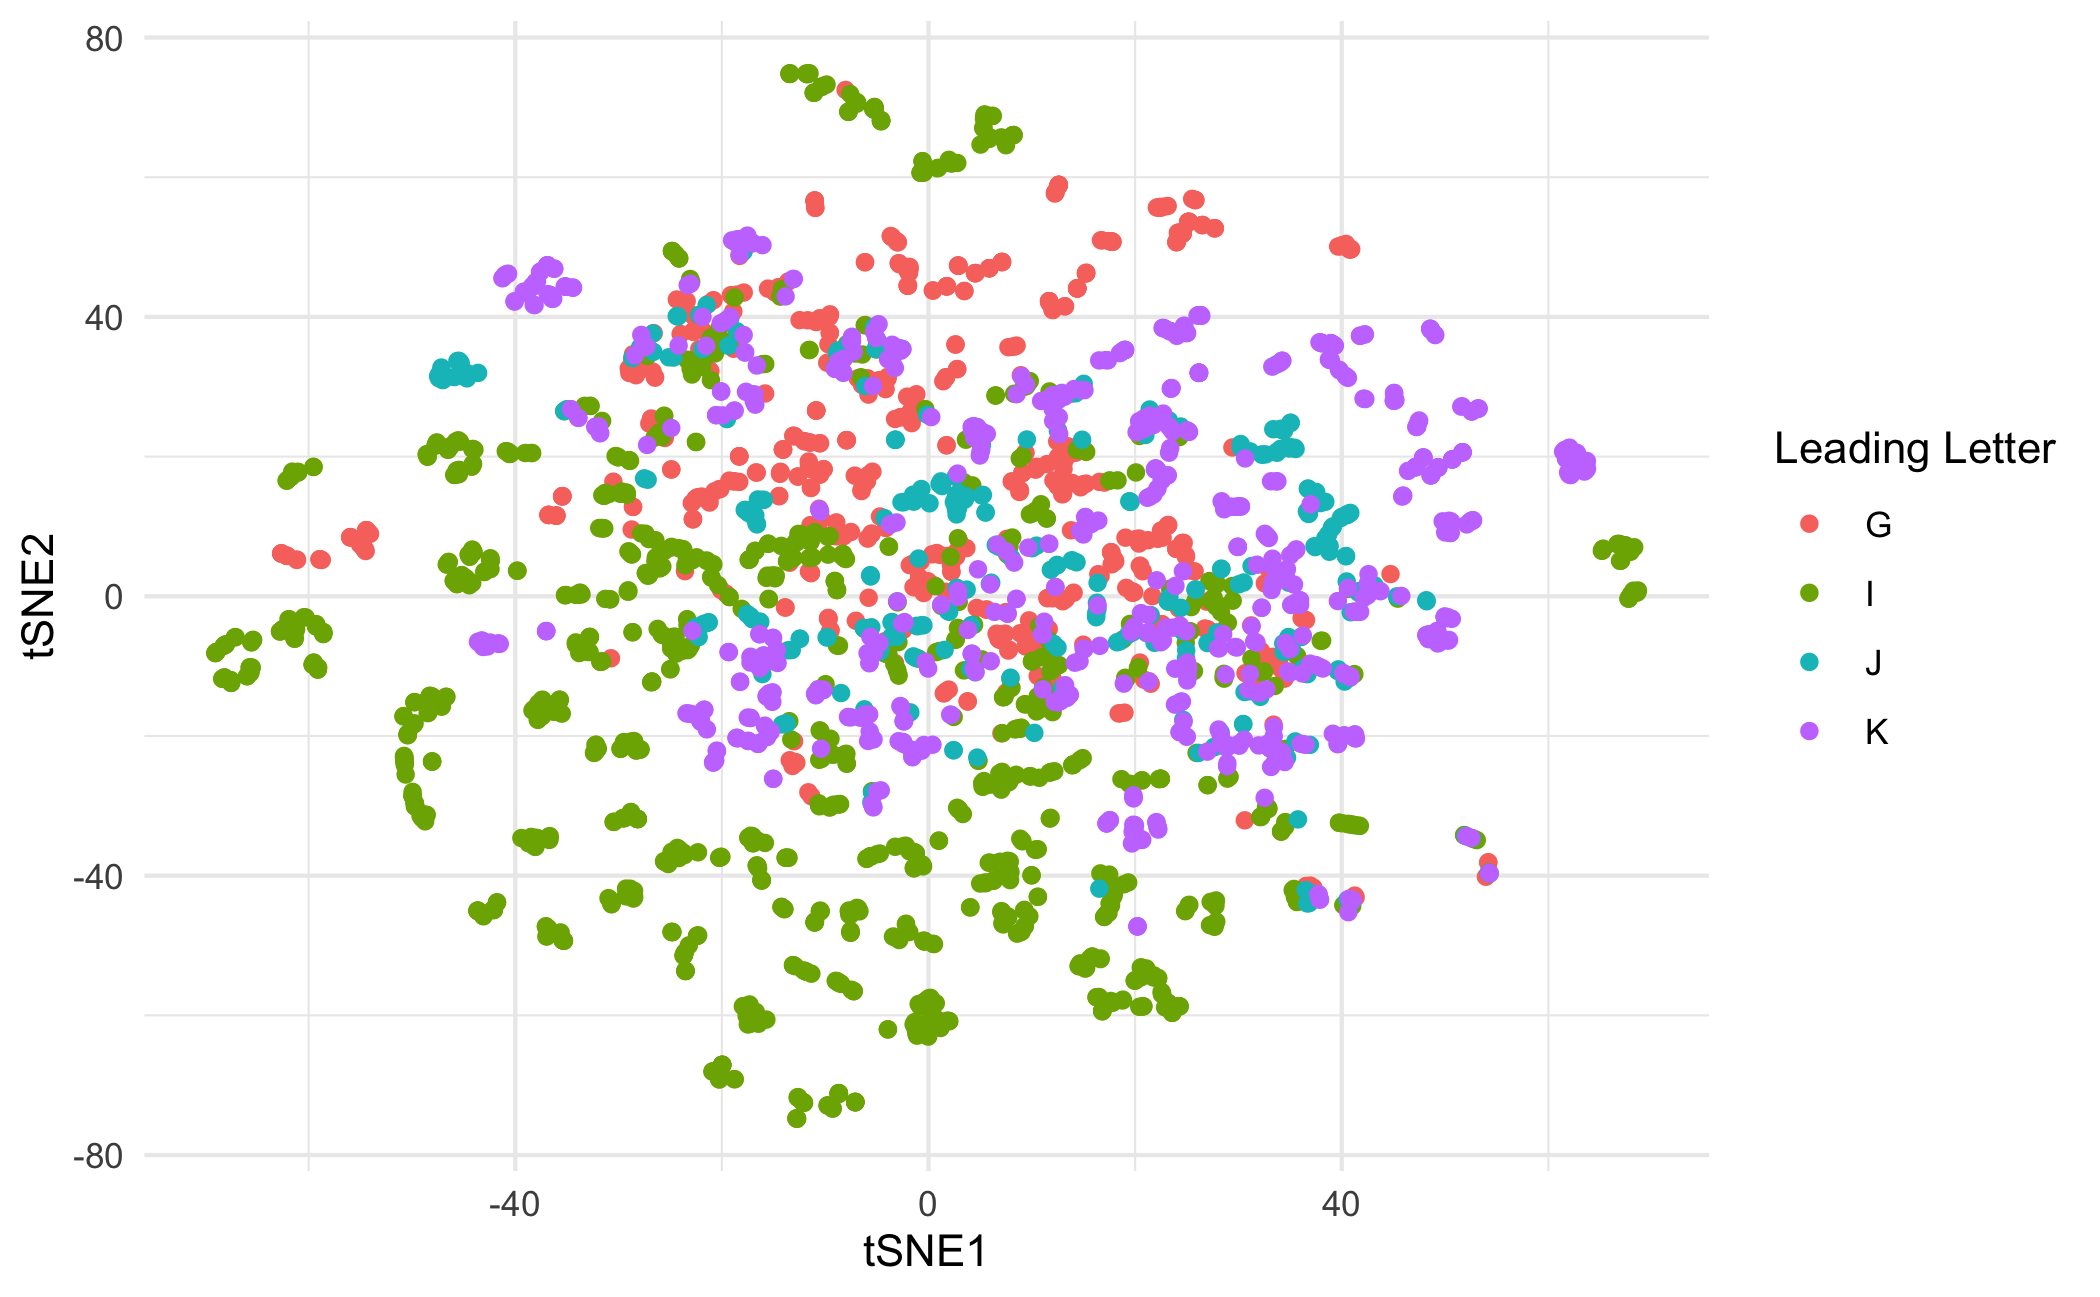
\includegraphics[width=\linewidth]{tsne-plot.png}
  \caption{The tSNE plot of the codes.}
  \label{fig:tsne}
\end{figure}

%%%%%%%%%%%%%%%%%%%%%%%%%%%%%%%%%%%
%%                               %%
%% Tables                        %%
%%                               %%
%%%%%%%%%%%%%%%%%%%%%%%%%%%%%%%%%%%

\pagebreak
%% Use of \listoftables is discouraged.
%%
\section*{Tables}

\begin{table}[ht!]
\caption{The autoencoder parameters and performance ordered by increasing validation loss.}
\label{tab:autoencoder_perf}
\begin{tabular}{|r|r|r|r|}
\hline
Embedding Dimension & Batch Size & Training Loss & Validation Loss\\
\hline
100 & 64 & 0.534 & 0.339\\
\hline
100 & 128 & 0.487 & 0.381\\
\hline
50 & 256 & 0.403 & 0.392\\
\hline
1000 & 64 & 0.542 & 0.402\\
\hline
100 & 256 & 0.556 & 0.444\\
\hline
1000 & 128 & 1.073 & 0.486\\
\hline
10 & 256 & 0.599 & 0.594\\
\hline
10 & 128 & 0.628 & 0.609\\
\hline
10 & 64 & 0.679 & 0.641\\
\hline
50 & 64 & 1.134 & 0.699\\
\hline
1000 & 256 & 30.435 & 0.803\\
\hline
50 & 128 & 1.053 & 0.894\\

\hline
\end{tabular}
\end{table}

\begin{table}[ht!]
\caption{The autoencoder validation performance ordered by year.}
\label{tab:autoencoder_year}
\begin{tabular}{|r|r|r|r|}
\hline
Year of Published ICD-10-CM Code& Embedding Dimension & Mean Square Error& Coef. of Determination\\
\hline
2019 & 10 & 0.593 & 0.086\\
\hline
2019 & 50 & 0.388 & 0.056\\
\hline
2019 & 100 & 0.336 & 0.049\\
\hline
2019 & 1000 & 0.400 & 0.058\\
\hline
2020 & 10 & 0.593 & 0.086\\
\hline
2020 & 50 & 0.388 & 0.056\\
\hline
2020 & 100 & 0.336 & 0.049\\
\hline
2020 & 1000 & 0.400 & 0.058\\
\hline
2021 & 10 & 0.594 & 0.086\\
\hline
2021 & 50 & 0.389 & 0.056\\
\hline
2021 & 100 & 0.337 & 0.049\\
\hline
2021 & 1000 & 0.401 & 0.058\\
\hline
2022 & 10 & 0.595 & 0.086\\
\hline
2022 & 50 & 0.390 & 0.056\\
\hline
2022 & 100 & 0.338 & 0.049\\
\hline
2022 & 1000 & 0.402 & 0.058\\
\hline
\end{tabular}
\end{table}

\begin{table}[ht!]
\caption{The supervised models' performance ordered by decreasing balanced accuracy.}
\label{tab:sup_perf}
\begin{tabular}{|r|r|r|r|}
\hline
Model & Embedding Dimension & Accuracy & Balanced Accuracy\\
\hline
BioGPT Compressed & 1000 & 0.960 & 0.927\\
\hline
BioGPT Compressed & 100 & 0.935 & 0.891\\
\hline
BioGPT Compressed & 50 & 0.925 & 0.873\\
\hline
BioGPT Compressed & 10 & 0.815 & 0.698\\
\hline
ClinicalBERT & 768 & 0.200 & 0.634 \\
\hline
PubMedBERT-MS-MARCO & 768 & 0.158 & 0.629\\
\hline
SapBERT-PubMedBERT & 768 & 0.159 & 0.616\\
\hline
MedBERT & 768 & 0.171 & 0.613\\
\hline
\end{tabular}
\end{table}


\pagebreak
%% Use of \listoftables is discouraged.
%%

\section*{Supplementary Materials}

\subsection{ICD-10-CM Category Codes}

\begin{table}[h]
%\caption{ICD-10-CM Category Codes.}
\begin{tabular}{l|l|}
\hline
Code & Description\\
\hline
S3559XS & Injury of other iliac blood vessels, sequela\\
\hline
M12262 & Villonodular synovitis (pigmented), left knee\\
\hline
S40011S & Contusion of right shoulder, sequela\\
\hline
K284 & Chronic or unspecified gastrojejunal ulcer with hemorrhage\\
\hline
M90632 & Osteitis deformans in neoplastic diseases, left forearm\\
\hline
\end{tabular}
\end{table}
%% Use of \listoftables is discouraged.
%%

\subsection*{ICD-10-CM Category Codes}

\begin{table}[ht!]
%\caption{ICD-10-CM Category Codes.}
\begin{tabular}{|l|l|l|}
\hline
First Code & Last Code & Code Description\\
\hline
A00 & B99 & Certain infectious and parasitic diseases\\
\hline
C00 & D49 & Neoplasms\\
\hline
D50 & D89 & Diseases of the blood and blood-forming organs and certain disorders \\
& & involving the immune mechanism\\
\hline
E00 & E89 & Endocrine, nutritional and metabolic diseases\\
\hline
F01 & F99 & Mental, Behavioral and Neurodevelopmental disorders\\
\hline
G00 & G99 & Diseases of the nervous system\\
\hline
H00 & H59 & Diseases of the eye and adnexa\\
\hline
H60 & H95 & Diseases of the ear and mastoid process\\
\hline
I00 & I99 & Diseases of the circulatory system\\
\hline
J00 & J99 & Diseases of the respiratory system\\
\hline
K00 & K95 & Diseases of the digestive system\\
\hline
L00 & L99 & Diseases of the skin and subcutaneous tissue\\
\hline
M00 & M99 & Diseases of the musculoskeletal system and connective tissue\\
\hline
N00 & N99 & Diseases of the genitourinary system\\
\hline
O00 & O9A & Pregnancy, childbirth and the puerperium\\
\hline
P00 & P96 & Certain conditions originating in the perinatal period\\
\hline
Q00 & Q99 & Congenital malformations, deformations and chromosomal abnormalities\\
\hline
R00 & R99 & Symptoms, signs and abnormal clinical and laboratory findings, not elsewhere classified\\
\hline
S00 & T88 & Injury, poisoning and certain other consequences of external causes\\
\hline
U00 & U85 & Codes for special purposes\\
\hline
V00 & Y99 & External causes of morbidity\\
\hline
Z00 & Z99 & Factors influencing health status and contact with health services\\
\hline
\end{tabular}
\end{table}



%%%%%%%%%%%%%%%%%%%%%%%%%%%%%%%%%%%
%%                               %%
%% Additional Files              %%
%%                               %%
%%%%%%%%%%%%%%%%%%%%%%%%%%%%%%%%%%%

%\section*{Additional Files}
%  \subsection*{Additional file 1 --- Sample additional file title}
%    Additional file descriptions text (including details of how to
%    view the file, if it is in a non-standard format or the file extension).  This might
%    refer to a multi-page table or a figure.
%
%  \subsection*{Additional file 2 --- Sample additional file title}
%    Additional file descriptions text.

\end{backmatter}
\end{document}
